\chapter{Psalm 80}

\begin{figure}
  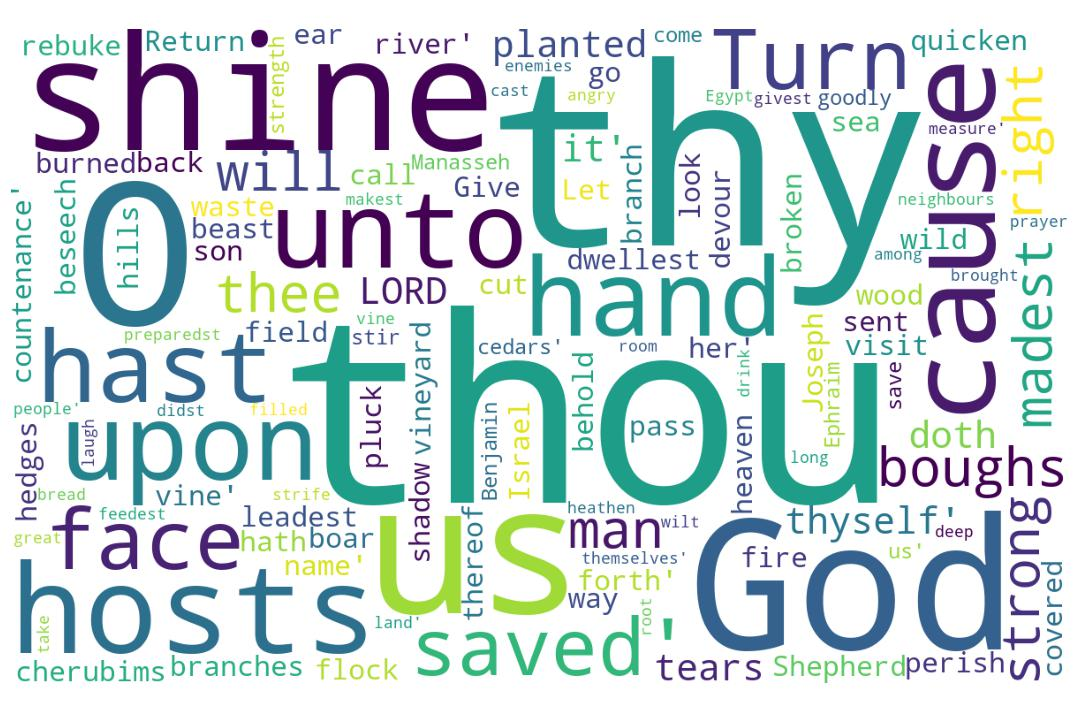
\includegraphics[width=\linewidth]{19OT-Psalms/Psalm80-WordCloud.jpg}
  \caption{Psalm 80 Word Cloud}
  \label{fig:Psalm 80 word Cloud}
\end{figure}

\marginpar{\scriptsize \centering \fcolorbox{bone}{lime}{\textbf{TURN US, LORD}}\\ (Psalm 80:1-19) \begin{compactenum}[I.][8]
     \item The \textbf{Envisioned Power} \index[scripture]{Psalms!Psa 080:01}(Psa 80:1)
     \item The \textbf{Vile and Vilified People} \index[scripture]{Psalms!Psa 080:06}(Psa 80:6)
     \item A \textbf{Vine Planted} \index[scripture]{Psalms!Psa 080:08}(Psa 80:8)
     \item A \textbf{Visit Proposed} \index[scripture]{Psalms!Psa 080:14}(Psa 80:14)
     \item A \textbf{Vineyard Pulled Down} \index[scripture]{Psalms!Psa 080:16}(Psa 80:16)
     \item The \textbf{Victor Empowered} \index[scripture]{Psalms!Psa 080:17}(Psa 80:17)
     \item The \textbf{Revitalized People} \index[scripture]{Psalms!Psa 080:19}(Psa 80:19)
\end{compactenum}}


\footnote{\textcolor[rgb]{0.00,0.25,0.00}{\hyperlink{TOC}{Return to end of Table of Contents.}}}
\footnote{\href{https://audiobible.com/bible/psalms_80.html}{\textcolor[cmyk]{0.99998,1,0,0}{Psalm 80 Audio}}}\textcolor[cmyk]{0.99998,1,0,0}{To the chief Musician upon Shoshannim-Eduth, A Psalm of Asaph.}\\
\\
\textcolor[cmyk]{0.99998,1,0,0}{Give ear, O Shepherd of Israel, thou that leadest Joseph like a flock; thou that dwellest \emph{between} the cherubims, shine forth.}
[2] \textcolor[cmyk]{0.99998,1,0,0}{Before Ephraim and Benjamin and Manasseh stir up thy strength, and come \emph{and} save us.}
[3] \textcolor[cmyk]{0.99998,1,0,0}{\fcolorbox{black}{red}{Turn us} again, O God, and cause thy face to shine; and we shall be saved.}
[4] \textcolor[cmyk]{0.99998,1,0,0}{O LORD God of hosts, how long wilt thou be angry against the prayer of thy people?}
[5] \textcolor[cmyk]{0.99998,1,0,0}{Thou feedest them with the bread of tears; and givest them tears to drink in great measure.}\footnote{\textbf{Deuteronomy 16:3} - Thou shalt eat no leavened bread with it; seven days shalt thou eat unleavened bread therewith, even the bread of affliction; for thou camest forth out of the land of Egypt in haste: that thou mayest remember the day when thou camest forth out of the land of Egypt all the days of thy life.}
[6] \textcolor[cmyk]{0.99998,1,0,0}{Thou makest us a strife unto our neighbours: and our enemies laugh among themselves.}
[7] \textcolor[cmyk]{0.99998,1,0,0}{\fcolorbox{black}{red}{Turn us} again, O God of hosts, and cause thy face to shine; and we shall be saved.}
[8] \textcolor[cmyk]{0.99998,1,0,0}{Thou hast brought a vine out of Egypt: thou hast cast out the heathen, and planted it.}
[9] \textcolor[cmyk]{0.99998,1,0,0}{Thou preparedst \emph{room} before it, and didst cause it to take deep root, and it filled the land.}
[10] \textcolor[cmyk]{0.99998,1,0,0}{The hills were covered with the shadow of it, and the boughs thereof \emph{were} \emph{like} the goodly cedars.}
[11] \textcolor[cmyk]{0.99998,1,0,0}{She sent out her boughs unto the sea, and her branches unto the river.}
[12] \textcolor[cmyk]{0.99998,1,0,0}{Why hast thou \emph{then} broken down her hedges, so that all they which pass by the way do pluck her?}
[13] \textcolor[cmyk]{0.99998,1,0,0}{The boar out of the wood doth waste it, and the wild beast of the field doth devour it.}
[14] \textcolor[cmyk]{0.99998,1,0,0}{Return, we beseech thee, O God of hosts: look down from heaven, and behold, and visit this vine;}
[15] \textcolor[cmyk]{0.99998,1,0,0}{And the vineyard which thy right hand hath planted, and the branch \emph{that} thou madest strong for thyself.}
[16] \textcolor[cmyk]{0.99998,1,0,0}{\emph{It} \emph{is} burned with fire, \emph{it} \emph{is} cut down: they perish at the rebuke of thy countenance.}
[17] \textcolor[cmyk]{0.99998,1,0,0}{Let thy hand be upon the man of thy right hand, upon the son of man \emph{whom} thou madest strong for thyself.}
[18] \textcolor[cmyk]{0.99998,1,0,0}{So will not we go back from thee: quicken us, and we will call upon thy name.}
[19] \textcolor[cmyk]{0.99998,1,0,0}{\fcolorbox{black}{red}{Turn us} again, O LORD God of hosts, cause thy face to shine; and we shall be saved.}\footnote{\textbf{Ezekiel 18:31} - Cast away from you all your transgressions, whereby ye have transgressed; and make you a new heart and a new spirit: for why will ye die, O house of Israel?}\footnote{\textbf{Ezekiel 36:26-28} - A new heart also will I give you, and a new spirit will I put within you: and I will take away the stony heart out of your flesh, and I will give you an heart of flesh. [27] And I will put my spirit within you, and cause you to walk in my statutes, and ye shall keep my judgments, and do them. [28] And ye shall dwell in the land that I gave to your fathers; and ye shall be my people, and I will be your God.}